\section{Theorie}
\label{sec:Theorie}

Um sowohl das Verhalten Ablenkverhalten von Elektronen in einem elektrischen, als auch in einem magnetischen Feld zu untersuchen, muss zunächst ein möglichst gebündelter Elektronenstrahl erzeugt werden.
Dies geschieht mittels einer Kathodenstrahlröhre, auf deren Aufbau in Kapitel \ref{sec:Versuchsaufbau} näher eingegangen wird.
Im Wesentlichen erzeugt sie über den glühelektrischen Effekt Elektronen, die über eine Anode beschleunigt werden.
Wichtig ist hierbei zu erwähnen, dass die gesamte Apparatur in einem Hochvakuum (bis ca. $\SI{e-6}{\milli\bar}$) sein muss, damit die Elektronen nicht mit Molekülen in Wechselwirkung treten und somit ihre eigentliche Bahn verfälschen.
Wenn die Elektronen die Anode passieren, sollten sie idealerweise eine kinetische Energie von
\begin{equation}
  E_{\text{kin}} = \frac{1}{2}m_0 v²_{\text{z}} = e_0 U_{\text{B}}
\end{equation}
haben.
Dabei beschreibt $U_{\text{B}}$ die Beschleunigungsspannung, $e_0$ und $m_0$ die Elektronenladung und -masse und $v_{\text{z}}$ dessen Geschwindigkeit in z-Richtung.
Demnach folgt der Ausdruck
\begin{equation}
  v_{\text{z}} = \sqrt{\frac{2 e_0 U_{\text{B}}}{m_0}}. \label{eqn:1}
\end{equation}

\subsection{Ablenkung des Elektronenstrahls mittels E-Feld}
Für weitere Erleuterungen wird das Schema \ref{fig:1} betrachtet.

\begin{figure}
  \centering
  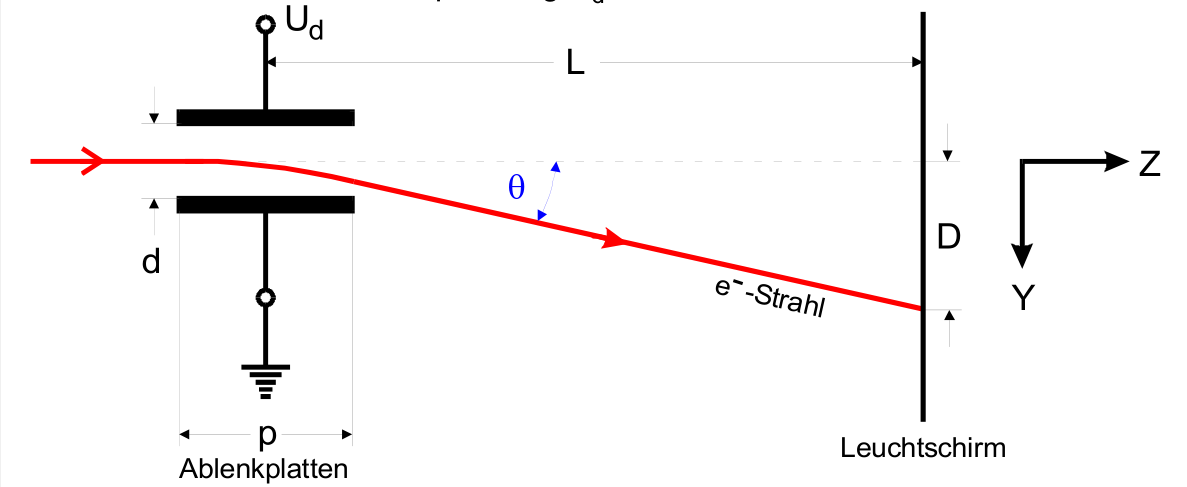
\includegraphics[height=4cm]{ressources/schema.png}
  \caption{Schematische Darstellung der Ablenkung mittels E-Feld. \cite{skript}}
  \label{fig:1}
\end{figure}

Passieren die Elektronen den Kondensator, werden sie durch das E-Feld vertikal abgelenkt.
Auf sie wirkt eine konstante Kraft von
\begin{equation}
  e_0 E = e_0 \frac{U_{d}}{d},
\end{equation}
wenn angenommen wird, dass der Plattenabstand $d$ klein gegenüber der Plattenlänge $p$ ist.
Durch die konstante Kraft führt das Elektron eine gleichmäßig beschleunigte Bewegung in y-Richtung aus.
Die Geschwindigkeit in jene Richtung, die es aufnimmt ist demnach
\begin{equation}
  v_{\text{y}} = \frac{F}{m_0} \increment{t},
\end{equation}
wobei
\begin{equation}
  \increment{t} = \frac{p}{v_{\text{z}}}
\end{equation}
die Zeit ist, in der sich ein Elektron zwischen den Platten aufhält.
Es ergibt sich
\begin{equation}
  v_{\text{y}} = \frac{e_0 U_d p}{m_0 d v_{\text{z}}}
\end{equation}
und da sich ein Elektron geradlinig gleichförmig nach Verlassen des Kondensators bewegt, folgt für den Ablenkwinkel
\begin{equation}
  \theta = \frac{v_{\text{y}}}{v_{\text{z}}}.
\end{equation}

Daraus lässt sich für die endgültige Ablenkung $D$ am Schirm die Formel
\begin{equation}
  D = L \theta = \frac{e_0}{m_0} \frac{U_d}{d} \frac{p}{v²_{\text{z}}} = L \frac{p}{2d} \frac{U_d}{U_{\text{B}}} \label{eqn:2}
\end{equation}
schreiben.\\
Um hochfrequente Wechselspannungen zu messen, muss $p$ möglichst klein und $U_{\text{B}}$ groß sein.
Dadurch wird jedoch die Ablenkung klein.
Die Kunst besteht demnach darin, einen guten Mittelweg zu finden.

\subsubsection{Kathodenstrahl-Oszillograph durch Ausnutzen der Ablenkeigenschaft}
Es ist durch die Ablenkeigenschaft, möglich einen Oszillographen zu realisieren, welcher eine Spannung in y-Richtung in Abhängigkeit von der Zeit in x-Richtung anzeigt.
Hierzu wird im Prinzip nur die Ablenkung in y-Richtung mit der zu untersuchenden Spannung gespeist.
Die Zeitachse wird durch eine Sägezahnspannung auf den Kondensator, welcher die Elektronen in x-Richtung ablenkt, gespeist.
Stehen die beiden Frequenzen der beiden Ablenkungen in einem bestimmten Verhältnis zueinander, können stehende Wellen beobachtet werden.
Dies ist der Fall, wenn das ganzzahlige Vielfache einer Frequenz durch ein ganzzahliges Vielfaches der anderen Frequenz darstellbar ist.
Jene Bedingung wird auch Synchronisationsbedingung genannt.

\subsection{Ablenkung des Elektronenstrahls mittels B-Feld}
Für die Kraft, welche auf die Elektronen wirkt, ist die Lorentzkraft
\begin{equation}
  F = e_0 \vec{v} \times \vec{B}
\end{equation}
für ein Elektron der Geschwindigkeit $v$ in einem Magnetfeld der Stärke $B$ zu beachten.
Bei einer reinen Geschwindigkeit in z-Richtung, sowie einem Magnetfeld in x-Richtung wird eine zu jeder Zeit senkrechte Ablenkung durch die Kraft
\begin{equation}
  F = e_0 v_{\text{z}} B
\end{equation}
realisiert.
Diese wirkt demnach wie eine Zentripetalkraft und es ergibt sich der Ausdruck
\begin{equation}
  e_0 v_0 B = \frac{m_0 v²_0}{r},
\end{equation}
wobei zu jeder Zeit $v_0 = v_{\text{z, Anfang}}$ gilt.
Nach Umformen nach dem Radius $r$ ergibt sich
\begin{equation}
  r = \frac{m_0 v_0}{e_0 B}. \label{eqn:3}
\end{equation}
\clearpage

\subsubsection{Bestimmung der spezifischen Elektronenladung}
Um die experimentelle Ablenkung des Elektronenstrahls untersuchen zu können, wird Schema \ref{fig:2} zur Hilfe genommen.
\begin{figure}
  \centering
  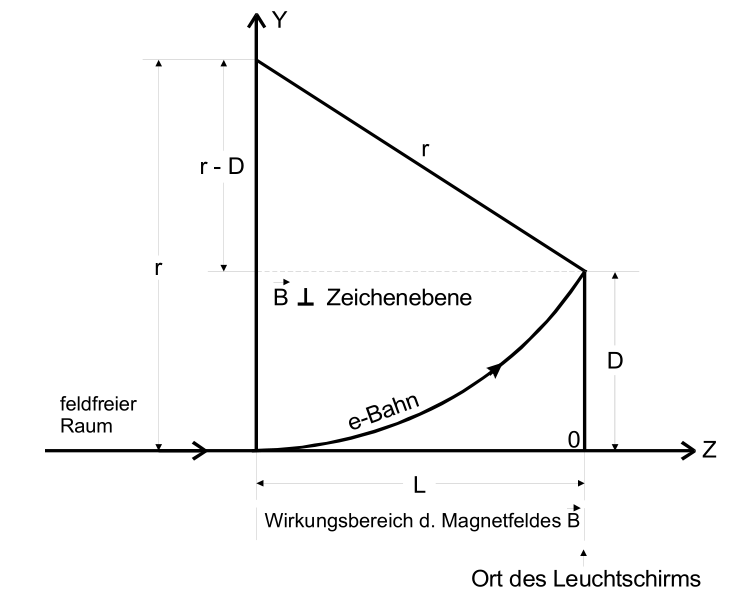
\includegraphics[height=4cm]{ressources/schema2.png}
  \caption{Schematische Darstellung der Ablenkung mittels B-Feld. \cite{skript}}
  \label{fig:2}
\end{figure}
Dabei folgt nach geometrischen Überlegungen (Satz des Pythagoras) für den Ablenkungradius des Elektronenstrahls im Wirkungsbereich des E-Feldes
\begin{equation}
  r = \frac{L²+D²}{2D}
\end{equation}
und nach Gleichsetzen mit Gleichung \eqref{eqn:3} nach Einsetzen der Beziehung \eqref{eqn:1} gilt für die spezifische Elektronenladung
\begin{equation}
  \frac{e_0}{m_0} = \frac{8 U_{\text{B}}}{B²} \frac{D²}{(L²+D²)²}. \label{eqn:4}
\end{equation}


% 2x2 Plot
% \begin{figure*}
%     \centering
%     \begin{subfigure}[b]{0.475\textwidth}
%         \centering
%         \includegraphics[width=\textwidth]{Abbildungen/Schaltung1.pdf}
%         \caption[]%
%         {{\small Schaltung 1.}}
%         \label{fig:Schaltung1}
%     \end{subfigure}
%     \hfill
%     \begin{subfigure}[b]{0.475\textwidth}
%         \centering
%         \includegraphics[width=\textwidth]{Abbildungen/Schaltung2.pdf}
%         \caption[]%
%         {{\small Schaltung 2.}}
%         \label{fig:Schaltung2}
%     \end{subfigure}
%     \vskip\baselineskip
%     \begin{subfigure}[b]{0.475\textwidth}
%         \centering
%         \includegraphics[width=\textwidth]{Abbildungen/Schaltung4.pdf}    % Zahlen vertauscht ... -.-
%         \caption[]%
%         {{\small Schaltung 3.}}
%         \label{fig:Schaltung3}
%     \end{subfigure}
%     \quad
%     \begin{subfigure}[b]{0.475\textwidth}
%         \centering
%         \includegraphics[width=\textwidth]{Abbildungen/Schaltung3.pdf}
%         \caption[]%
%         {{\small Schaltung 4.}}
%         \label{fig:Schaltung4}
%     \end{subfigure}
%     \caption[]
%     {Ersatzschaltbilder der verschiedenen Teilaufgaben.}
%     \label{fig:Schaltungen}
% \end{figure*}
